\subsection{Einführung}

\begin{problem}
Gegeben $f: [a,b] \rightarrow \mathbb{N}$ mit $a, b \in \mathbb{R}$.
Berechne $\int_a^b f(x) dx $
\end{problem}

\begin{example}
\begin{description}
  \item 
\end{description}
\begin{enumerate}
  \item Archimedes (282-212 v.Chr.): Fläche unter einer Parabel \\ \\
    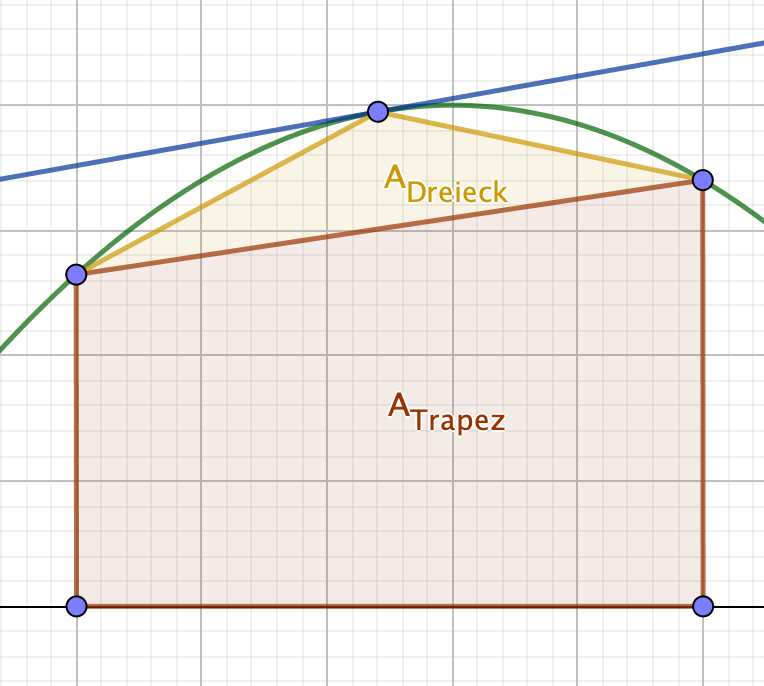
\includegraphics[width=5cm]{Kapitel_1/Grafiken/Grafik_1.png} \\
    $A_{Parabel} = A_{Trapez} + \frac{4}{3} A_{Dreieck}$
  \item Leibniz + Newton (~1670):
    $$ \int_a^b f(x) dx = F(b) - F(a),$$ wobei $\frac{d}{dx} F(x) = f(x)$
  \item Riemann (~1850): 
    $$ \int_a^b f(x) dx = \lim\limits_{\vert \Delta \vert \to \infty} \sum_{j=1}^n f(\xi_j)(x_j - x_{j-1}),$$
    wobei $\Delta = (x_0,...,x_n)$ Gitter Zerlegung von $[a, b]$, $a=x_0 < ...< x_n = b$, $\xi_j \in [x_{j-1}, x_j]$ und $\vert \Delta \vert := \max_{j=1,...n} \vert x_j - x_{j-1} \vert$.
    Das Riemannintegral existiert, falls: 
    $$ \forall \varepsilon > 0 \exists \delta > 0: \vert \Delta \vert < \delta \Rightarrow \vert \int_a^b f(X) dx - \sum_{j=1}^n f(\xi_j)(x_j-x_{j-1}) \vert < \varepsilon $$
\end{enumerate}
\end{example}

\begin{comment}[Approximation von Integralen]
\begin{description}
  \item 
\end{description}
\begin{enumerate}
  \item (linke) Rechtecksregel: 
    $$\int_{x_{j-1}}^{x_{j-1}+h} f(x) dx \approx h f(x_{j-1})$$
    $$\int_a^b f(x) dx = \sum_{j=1}^n \int_{x_{j-1}}^{x_j} f(x)dx \approx \sum_{j=1}^n f(x_{j-1}) (x_j-x_{j-1})$$
  \item Mittelpunktsregel:
    $$\int_{x_{j}}^{x_{j}+h} f(x) dx \approx f\left(\frac{x_j+x_j+h}{2}\right)h$$
    $$\int_a^bf(x)dx \approx \sum_{j=1}^n f\left( \frac{x_{j-1} + x_j}{2}\right) (x_j - x_{j-1})$$
    Da mit Hilfe der Transformationsformel sich jedes Integral $\int_{x_{j-1}}^{x_j}$ auf ein Integral $\int_a^b$ transformieren lässt, betrachten wir ohne Einschränkungen Integrale von $0$ bis $1$. Nutze dazu die Abb. $[a, b] \rightarrow [x_{j-1}, x_j], t \mapsto x_{j-1} + t(x_j - x_{j-1})$.
    $$ \int_{x_{j-1}}^{x_j} f(x) dx = \int_0^1 \underbrace{f\left( x_{j-1} + t(x_j - x_{j-1})\right)}_{:= g_{j-1}(t)} (x_j - x_{j-1})dt = \int_0^1 g_{j-1}(t)(x_j-x_{j-1})dt$$
\end{enumerate}
\end{comment}

\begin{definition}[Quadraturformel]
Eine s-stufige Quadraturformel zur Approximation von $\int_0^1 g(t)dt$ mit Knoten $c_i$ und Gewichten $b_i$ für $i=1,...s$ ist gegeben durch 
$$\sum_{i=1}^s b_i g(c_i) \left( \approx \int_0^1 g(t) dt\right)$$

\end{definition}

\begin{example}
\begin{description}
  \item 
\end{description}
\begin{enumerate}
  \item Rechtecksregel: $s = 1, b_1 = 1, c_1 = 0$
    $$ \int_0^1 g(t) \approx b_1 g(c_1) = g(0)$$
  \item Mittelpunktsregel: $s = 1, b_1 = 1, c_1 = \frac{1}{2}$
    $$ \int_0^1 g(t) \approx g(\frac{1}{2})$$
  \item Trapezregel: $s=2, b_1=b_2= \frac{1}{2}, c_1 = 0, c_2 = 1$
    $$ \int_0^1 g(t) \approx \frac{1}{2} g(0) + \frac{1}{2}g(1)$$
  \item Simpsonregel: $s=3, b_1 =  \frac{1}{6}, b_2 =  \frac{2}{3}, b_3 =  \frac{1}{6}, c_1 = 0, c_2 =  \frac{1}{2}, c_3 = 1$
    $$ \int_0^1 g(t) \approx \frac{1}{6} \left(g(0) + 4g\left(\frac{1}{2}\right) +g(1)\right)$$ 
    \textbf{Herleitung:} Man legt eine Parabel $p$ durch die Punkte $(0, g(0)), (\frac{1}{2}, g(\frac{1}{2})), (1, g(1))$ und integriert $p$ von 0 bis 1. \\
    $p(t) = g(0)(1-t)2(\frac{1}{2}-t) + g(\frac{1}{2})(1-t)4t + g(1)(\frac{1}{2}-t)2t$ \\
    $$\Rightarrow \int_0^1 p(t)dt = \frac{1}{6}g(0)+ \frac{2}{3}g(\frac{1}{2}) +\frac{1}{6}g(1)$$ 
  \item "pulcherrima et utilissima regula" von Newton:
    $$\int_0^1 g(t) dt \approx \frac{1}{8}\left(g(0) + 3g(\frac{1}{3}) + 3g(\frac{2}{3}) + g(1)\right)$$
\end{enumerate}

\end{example}

\begin{comment}[Monte-Carlo Integration]
\begin{description}
  \item 
\end{description}
\begin{enumerate}
  \item Eindimensionale Monte-Carlo Integration: \\
    Sei $a, b \in \mathbb{R}$, $a<b$. Wählt man $N$ unabhängige gleichverteilte Punkte $x_i$ in $[a,b]$ so gilt die Approximation:
    $$\int_a^b f(x) dx \approx \frac{1}{N} \sum_{j=1}^N (b-a)f(x_j)$$
    Nach dem Gesetz der großen Zahlen konvergiert dieser Ausdruck, falls 
    $$\int_a^b\vert f(x) \vert dx < \infty, \int_a^b f^2(x)dx < \infty$$
  \item Mehrdimensionale Monte-Carlo Integration: \\
    Sei $W=\otimes_{i=1}^d [a_i, b_i]$ ein d-dimensionaler Quader. Wählt man in W unabh. gleichvert. Zufallsvektoren $x_i$ in W, so ist
    $$\int_W f(x)dx \approx \frac{1}{N} Vol(W) \sum_{i=1}^N f(x_i),$$
    wobei $f:\mathbb{R}^d \rightarrow \mathbb{R}$.\\
    \textbf{Achtung:} Dieses gewöhnliche MC-Verfahren konvergiert sehr langsam. Verbesserungen sind z.B.: Importance sampling, Control variates, Antithetic variates und statified sampling.
\end{enumerate}
\end{comment}